\documentclass[11pt,a4paper]{article}
\usepackage[margin=2.2cm]{geometry}
\usepackage{amsmath,amssymb,amsfonts}
\usepackage{booktabs,array,tabularx}
\usepackage{enumitem}
\usepackage[table]{xcolor}
\usepackage{tikz}
\usetikzlibrary{arrows.meta,positioning,shapes.geometric,calc}
\usepackage[colorlinks=true,linkcolor=blue!50!black,urlcolor=blue!50!black]{hyperref}
\usepackage{titlesec}
\titleformat{\section}{\large\bfseries}{\thesection}{0.8em}{}
\titleformat{\subsection}{\normalsize\bfseries}{\thesubsection}{0.8em}{}
\setlength{\parindent}{0pt}
\setlength{\parskip}{5pt}

\newcommand{\I}{\mathcal{I}}
\newcommand{\F}{\mathcal{F}}
\newcommand{\G}{\mathcal{G}}
\newcommand{\M}{\mathcal{M}}
\newcommand{\N}{\mathcal{N}}
\newcommand{\A}{\mathcal{A}}
\newcommand{\Rs}{\text{Rs}\,}

% coloured boxes without extra packages
\newcommand{\cbox}[3]{\par\noindent\fcolorbox{#1!55!black}{#1!6}{\begin{minipage}{\dimexpr\linewidth-2\fboxsep-2\fboxrule\relax}#3\end{minipage}}\par\vspace{2pt}}
\newcommand{\idea}[1]{\cbox{blue}{}{\textbf{Key idea.} #1}}
\newcommand{\plain}[1]{\cbox{green}{}{\textbf{In plain words.} #1}}
\newcommand{\without}[1]{\cbox{red}{}{\textbf{What goes wrong without it.} #1}}
\newcommand{\toy}[1]{\cbox{orange}{}{\textbf{In the toy example (Section~\ref{sec:toy}).} #1}}

\title{\textbf{F2 explained}\\[3pt]
\large The continuous-time MILP for EV charging: FCS assignment + mobile charger routing\\[2pt]
\normalsize A step-by-step guide to \texttt{F2\_continuous\_time\_MILP.pdf}, with a worked example}
\author{CP 320 OR for Mobility Management, course project}
\date{14 October 2026 (matches the dataset-independent revision of F2)}

\begin{document}
\maketitle

\textbf{How to read this.} Section~\ref{sec:story} tells the problem as a story. Section~\ref{sec:ideas} gives the five modelling ideas that turn the city into equations; if you understand these, the rest is bookkeeping. Sections~\ref{sec:inputs}--\ref{sec:cons} go through every input, variable, cost term and constraint of F2. Each constraint has its formula, a plain-words reading and what would break without it. Section~\ref{sec:toy} solves a five-EV example completely, with a map and a timeline. Section~\ref{sec:cheat} is a one-page summary to keep next to you while coding.

Equation tags like \textbf{(F2-4)} are the equation numbers in \texttt{F2\_continuous\_time\_MILP.pdf}, so you can look each one up there.

\tableofcontents
\newpage

%=====================================================================
\section{The story}\label{sec:story}

It is the evening peak, from time $0$ to time $T$. Across the city, EV drivers ask to have their car charged. Request $i$ comes in at time $r_i$, needs $E_i$ kWh, and the driver would like the car ready by $l_i$. The car has $R_i$ km of range left.

The operator has two kinds of resources:
\begin{itemize}[leftmargin=1.4em,itemsep=2pt]
  \item \textbf{Fixed charging stations (FCS).} Each has 2 guns of 22\,kW. An EV sent to an FCS \emph{drives there itself}, waits if both guns are busy, and charges.
  \item \textbf{Mobile charging vans (MCS).} A van leaves the depot, drives to a parked EV, charges it, drives to the next EV, and so on, then returns to the depot. A van charges \emph{one EV at a time}, and both its driving and the energy it delivers come out of one battery of $B_m$ kWh.
\end{itemize}

F2 answers three questions at once:
\begin{enumerate}[leftmargin=1.6em,itemsep=2pt]
  \item \textbf{Who} serves each EV: which gun of which station, or which van?
  \item In \textbf{what order} does each van visit its EVs (and each gun charge its EVs)?
  \item \textbf{When} does each charging session start?
\end{enumerate}
The answer must serve \emph{every} EV by $T$ and make
\[
\text{operating cost} \;+\; \text{customer inconvenience (in rupees)}
\]
as small as possible.

\idea{Questions 1 and 2 are the two questions in the project brief. Question 3 is what makes F2 \emph{continuous-time}: it does not just count how many EVs a station gets, it schedules them on a clock. That is how it can see queues at a station and the time a van needs to reach an EV.}

%=====================================================================
\section{Five modelling ideas}\label{sec:ideas}

\subsection*{Idea 1: work on a small graph of key places, not on the streets}
The model only needs distances between a few places: the depot, the $n$ EVs and the stations. These are computed \emph{once, before solving}, from whatever data you have: straight-line distance between coordinates (times a detour factor), or shortest paths on a road map. The model does not care where they come from. In the model they are just numbers: $d_{if},t_{if}$ (EV $i$ to station $f$) and $d_{ij},t_{ij}$ (between depot and EVs, for vans). Travel time is $t=d/v$.

\subsection*{Idea 2: the depot appears twice, as 0 and $n+1$}
A van route is a chain of arcs \emph{start depot $\to$ EV $\to$ EV $\to\dots\to$ end depot}. Node $0$ is ``leave the depot'' and node $n+1$ is ``come back to the depot''. They are the same place. Splitting them makes every route a simple path from $0$ to $n+1$, which is easy to describe with flow constraints. A variable $x_{ijm}=1$ means ``van $m$ drives straight from $i$ to $j$''.

\subsection*{Idea 3: every gun is a machine, like in machine scheduling}
A station with 2 guns is treated as 2 separate machines. Each EV sent to the station goes onto \emph{one} gun ($y_{ig}=1$). Two EVs on the same gun must not overlap in time. This is the classical ``either $i$ before $j$, or $j$ before $i$'' rule, written with a binary $o_{ij}$. Once each gun runs at most one EV at a time, the station automatically never has more than 2 EVs charging.

\subsection*{Idea 4: one clock value per EV}
Every EV gets one start time $S_i$, whichever resource serves it. Its completion time is then
\[
C_i = S_i + \underbrace{\tau^F_i\textstyle\sum_g y_{ig}}_{\text{if at an FCS}} + \underbrace{\tau^M_i\textstyle\sum_m z_{im}}_{\text{if by a van}}, \qquad \tau^F_i=\frac{E_i}{P^F},\ \tau^M_i=\frac{E_i}{P^M}.
\]
Exactly one of the two sums is 1, so $C_i$ is ``start + duration on the chosen resource''. With one $S_i$ for everyone, ``how long did the driver wait'' is measured the same way for FCS and van customers: $C_i-r_i$.

\subsection*{Idea 5: range decides which stations are even allowed}
EV $i$ can only drive to stations within its remaining range: $\F_i=\{f: d_{if}\le R_i\}$, and $\G_i$ is the set of guns at those stations. Variables $y_{ig}$ exist \emph{only} for $g\in\G_i$. If $\F_i$ is empty, the EV has no FCS option at all and the model must send a van. This is how stranded, low-battery EVs are protected without any special rule.

%=====================================================================
\section{Inputs: sets and parameters}\label{sec:inputs}

\subsection{Sets (the ``things'' in the model)}
\begin{tabularx}{\textwidth}{@{}lX@{}}
\toprule
$\I=\{1,\dots,n\}$ & EV charging requests \\
$\F$ & fixed stations; $\G_f$ = the 2 guns of station $f$; $\G$ = all guns; $f(g)$ = the station gun $g$ belongs to \\
$\F_i,\ \G_i$ & stations / guns EV $i$ can reach (Idea 5) \\
$\M$ & vans \\
$\N=\{0\}\cup\I\cup\{n+1\}$ & routing nodes (Idea 2) \\
$\A$ & van arcs $(i,j)$: from the start depot or an EV, to an EV or the end depot, $i\ne j$, and not $0\to n+1$ directly (an unused van simply has no arcs) \\
$\mathcal{P}_g$ & pairs $(i,j)$, $i<j$, that are \emph{both} allowed on gun $g$; only these pairs need a ``who goes first'' decision \\
\bottomrule
\end{tabularx}

\subsection{Parameters (numbers you give the model)}
\begin{tabularx}{\textwidth}{@{}l>{\raggedright\arraybackslash}p{6.2cm}X@{}}
\toprule
\textbf{Symbol} & \textbf{Meaning} & \textbf{Value used in the toy example} \\
\midrule
$E_i,\ r_i,\ l_i,\ R_i$ & energy (kWh), request time, desired-ready time (h), range left (km) & see Table~\ref{tab:toydata} \\
$w_i\ge1$ & priority: $w_i=1+\kappa(1-R_i/R_{\max})$, low range $\Rightarrow$ high priority & $\kappa=2$, $R_{\max}=40$ \\
$P^F,\ P^M$ & charging power of a gun / of a van & 22\,kW / 30\,kW \\
$\tau^F_i,\ \tau^M_i$ & charging time at an FCS / by a van, $E_i/P$ & computed \\
$v$ & travel speed & 25\,km/h \\
$B_m,\ Q_m$ & van battery, max EVs per van per period & 150\,kWh, 6 \\
$\beta,\ \eta$ & van driving use (kWh/km), charging efficiency & 0.25, 0.9 \\
$T$ & horizon length & 4\,h \\
$c^{EV},\ c^M$ & cost per km of EV driving / van driving & \Rs4, \Rs15 \\
$c^F_m$ & fixed cost of sending van $m$ out & \Rs1500 \\
$\pi^F,\ \pi^M$ & cost per kWh at an FCS (grid) / from a van battery & \Rs8.7, \Rs10.7 \\
$c^W$ & cost of one hour that a car is not ready (``value of time'') & \Rs200/h \\
$c^L$ & cost of one hour beyond $l_i$ & \Rs300/h \\
\bottomrule
\end{tabularx}

These are the illustrative values from F2 Section~3.3. They are starting points for experiments, not part of the model.

\idea{F2 is \textbf{not tied to any dataset}. An instance is just this list of numbers: EV locations, $E_i,r_i,l_i,R_i$, station locations, van data, costs and a distance/time matrix. You can make them up by hand (as in the toy example below), generate them randomly, or take them from real data. Only the numbers change, never the model.}

%=====================================================================
\section{Decision variables (what the solver chooses)}\label{sec:vars}

\begin{tabularx}{\textwidth}{@{}lllX@{}}
\toprule
\textbf{Var.} & \textbf{Type} & \textbf{Answers} & \textbf{Meaning} \\
\midrule
$y_{ig}$ & 0/1 & who? & EV $i$ is charged on gun $g$ (only for $g\in\G_i$) \\
$z_{im}$ & 0/1 & who? & EV $i$ is charged by van $m$ \\
$x_{ijm}$ & 0/1 & order (van) & van $m$ drives straight from $i$ to $j$ \\
$u_m$ & 0/1 & & van $m$ leaves the depot at all \\
$o_{ij}$ & 0/1 & order (gun) & if $i$ and $j$ end up on the same gun: 1 if $i$ goes first, 0 if $j$ goes first \\
$S_i$ & $\ge0$ & when? & time charging of EV $i$ starts (h) \\
$L_i$ & $\ge0$ & & hours EV $i$ is late beyond $l_i$ \\
\bottomrule
\end{tabularx}

\textbf{Short-hands} (not new variables, just names for sums):
\[
Y_{if}=\sum_{g\in\G_f}y_{ig}\ \ (\text{EV $i$ goes to station $f$}),\qquad
C_i=S_i+\tau^F_i\sum_{g\in\G_i}y_{ig}+\tau^M_i\sum_{m}z_{im}\ \ (\text{ready time}).
\]

\idea{The binaries do the \emph{combinatorial} work (who, which order). The continuous $S_i$ do the \emph{clock} work. Big-M constraints connect the two: a timing rule is switched on only when the binaries say it applies.}

%=====================================================================
\section{The objective, term by term}\label{sec:obj}

\begin{align*}
\min\ Z \;=\;& \underbrace{c^{EV}\sum_{i}\sum_{f\in\F_i} d_{if}\,Y_{if}}_{Z_1:\ \text{EV driving}}
\;+\; \underbrace{c^{M}\sum_{m}\sum_{(i,j)\in\A} d_{ij}\,x_{ijm}}_{Z_2:\ \text{van driving}}
\;+\; \underbrace{\sum_{m} c^{F}_m\,u_m}_{Z_3:\ \text{van dispatch}} \\[2pt]
&+\; \underbrace{\pi^F\sum_{i}\sum_{g\in\G_i} E_i\,y_{ig} \;+\; \pi^M\sum_{i}\sum_{m}\frac{E_i}{\eta}\,z_{im}}_{Z_4:\ \text{energy}}
\;+\; \underbrace{c^W\sum_{i} w_i\,(C_i - r_i)}_{Z_5:\ \text{inconvenience}}
\;+\; \underbrace{c^L\sum_{i} w_i\,L_i}_{Z_6:\ \text{lateness}} \tag{F2-1}
\end{align*}

\begin{tabularx}{\textwidth}{@{}l>{\raggedright\arraybackslash}p{5.6cm}X@{}}
\toprule
\textbf{Term} & \textbf{What it counts} & \textbf{Which way it pushes} \\
\midrule
$Z_1$ & km each FCS customer drives to its station & towards the \emph{nearest} station; against far stations \\
$Z_2$ & km of all van routes & short routes; EVs close together on the same van \\
$Z_3$ & fixed cost of each van that goes out & as few vans as possible \\
$Z_4$ & energy: grid kWh at FCS vs van kWh ($1/\eta$ more is drawn, at a higher price) & towards the FCS: a van kWh costs $10.7/0.9=\Rs11.9$, a grid kWh \Rs8.7 \\
$Z_5$ & priority-weighted hours from request to ready & against queues and slow vans; serve high-$w_i$ EVs first; use a van if the gun queue is long \\
$Z_6$ & priority-weighted hours late beyond $l_i$ & finish before the driver needs the car \\
\bottomrule
\end{tabularx}

\plain{$Z_1$--$Z_4$ are the operator's costs and favour the FCS. $Z_5$--$Z_6$ are the drivers' costs and favour whatever is fastest, often the van. The optimum is the best balance. Change $c^W$ and $c^L$ and you move along the trade-off between a cost-first and a customer-first operator.}

\textbf{Why $Z_5$ is linear even though waiting depends on the route.} $C_i-r_i$ is a linear expression in $S_i$, $y$ and $z$. The constraints force $S_i$ to the true start time, so the waiting is exact. The part $c^W\sum_i w_ir_i$ is a constant and can be dropped while solving; add it back when you report $Z$.

\textbf{Why $L_i$ equals the real lateness.} Constraint (F2-19) says $L_i\ge C_i-l_i$, and $L_i\ge0$. Because $L_i$ costs money in $Z_6$, the solver makes it as small as allowed: $L_i=\max\{0,\,C_i-l_i\}$.

%=====================================================================
\section{The constraints, one by one}\label{sec:cons}

\subsection{Everybody is served exactly once}
\begin{equation}
\sum_{g\in\G_i} y_{ig} + \sum_{m\in\M} z_{im} = 1 \qquad \forall i \tag{F2-2}
\end{equation}
\plain{Each EV gets exactly one gun of one reachable station, or exactly one van. If $\G_i$ is empty (no station within range), the first sum is empty and some $z_{im}$ must be 1: the EV is forced onto a van.}
\without{An EV could be left out (cost 0, cheapest!) or served twice. This is the ``all requests satisfied'' KPI of the brief.}

\subsection{You cannot charge before you arrive}
\begin{equation}
S_i \ \ge\ r_i + \sum_{f\in\F_i} t_{if}\,Y_{if} \qquad \forall i \tag{F2-3}
\end{equation}
\plain{An FCS customer starts at the earliest after the request plus the drive to the chosen station. For a van customer all $Y_{if}=0$ and this reads $S_i\ge r_i$.}

\subsection{No two EVs on the same gun at the same time (the disjunctive pair)}
\begin{align}
S_j &\ \ge\ S_i + \tau^F_i - (T+\tau^F_i)\,(3 - y_{ig} - y_{jg} - o_{ij}) && \forall g,\ (i,j)\in\mathcal{P}_g \tag{F2-4}\\
S_i &\ \ge\ S_j + \tau^F_j - (T+\tau^F_j)\,(2 - y_{ig} - y_{jg} + o_{ij}) && \forall g,\ (i,j)\in\mathcal{P}_g \tag{F2-5}
\end{align}
This is the heart of the FCS part. Read the bracket as a switch: when it is $0$ the constraint is \emph{on}, when it is $\ge1$ the big term makes it \emph{off} (always true).

\begin{center}
\renewcommand{\arraystretch}{1.25}
\begin{tabular}{@{}ccc|cc|l@{}}
\toprule
$y_{ig}$ & $y_{jg}$ & $o_{ij}$ & bracket in (F2-4) & bracket in (F2-5) & result \\
\midrule
1 & 1 & 1 & 0 $\to$ \textbf{on} & 1 $\to$ off & $S_j\ge S_i+\tau^F_i$: $i$ finishes, then $j$ starts \\
1 & 1 & 0 & 1 $\to$ off & 0 $\to$ \textbf{on} & $S_i\ge S_j+\tau^F_j$: $j$ finishes, then $i$ starts \\
1 & 0 & any & $\ge1$ $\to$ off & $\ge1$ $\to$ off & not on the same gun: no link \\
0 & 0 & any & $\ge2$ $\to$ off & $\ge2$ $\to$ off & no link \\
\bottomrule
\end{tabular}
\end{center}

\textbf{Why $T+\tau^F_i$ is a big enough ``big-M''.} When switched off, (F2-4) reads $S_j\ge S_i+\tau^F_i-(T+\tau^F_i)\cdot1=S_i-T$. Since $S_i\le T$ and $S_j\ge0$, this is always true, so it really is off. A bigger M would also be correct but makes the LP relaxation weaker and the solver slower; this is the smallest safe value.

\plain{If two EVs share a gun, the solver must pick an order, and the second one waits until the first is done. With 2 guns per station, at most 2 EVs charge at a station at any moment. No time grid is needed.}
\without{Both EVs would charge on one gun at the same time, so a station could serve unlimited EVs in parallel and there would never be a queue.}

\subsection{A tightening cut: total work per gun (optional)}
\begin{equation}
\sum_{i}\tau^F_i\,y_{ig} \ \le\ T - \min_{i:\,g\in\G_i}\,(r_i+t_{i f(g)}) \qquad \forall g \tag{F2-6}
\end{equation}
\plain{The charging hours placed on one gun must fit in the time that gun can be used, from the first possible arrival until $T$.}
This is already implied by (F2-3)--(F2-5). Adding it does not change the optimum but helps the solver, because the LP relaxation (binaries allowed to be fractional) can otherwise ignore the switches. On its own, without (F2-4)--(F2-5), it gives a fast but rough \emph{capacity-only} model: that is essentially what F4 uses.

\subsection{The two guns are identical (optional)}
\begin{equation}
\sum_i y_{ig_1} \ \ge\ \sum_i y_{ig_2} \qquad \forall f,\ \G_f=\{g_1,g_2\} \tag{F2-7}
\end{equation}
\plain{Swapping all EVs between gun 1 and gun 2 of a station gives the same plan. This rule keeps only one of the two mirror images (gun 1 gets at least as many EVs), so branch-and-bound explores half as much.}

\subsection{Van routes: leave once, return once, visit each own EV once}
\begin{align}
\sum_{j} x_{0jm} &= u_m, \qquad \sum_{i} x_{i,n+1,m} = u_m && \forall m \tag{F2-8, 9}\\
\sum_{i} x_{ijm} &= z_{jm}, \qquad \sum_{k} x_{jkm} = z_{jm} && \forall j\in\I,\ m \tag{F2-10, 11}
\end{align}
\plain{A van that is used leaves the depot on exactly one arc and comes back on exactly one arc; an unused van has no arcs. An EV given to van $m$ is entered once and left once \emph{by that van}; any other van never touches it. This links the routing ($x$) to the assignment ($z$).}

\begin{center}
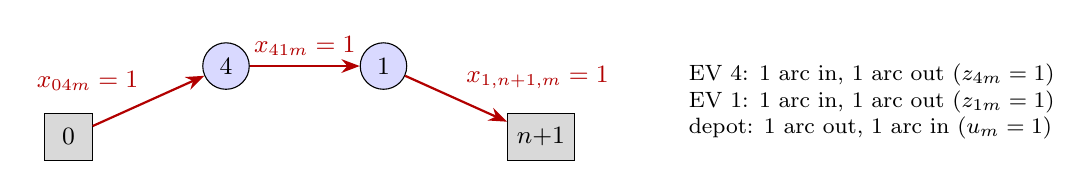
\begin{tikzpicture}[>=Stealth, every node/.style={font=\small}]
  \node[draw,fill=black!15,minimum size=6mm] (D0) at (0,0) {0};
  \node[circle,draw,fill=blue!15] (a) at (2,0.9) {4};
  \node[circle,draw,fill=blue!15] (b) at (4,0.9) {1};
  \node[draw,fill=black!15,minimum size=6mm] (D1) at (6,0) {$n{+}1$};
  \draw[->,thick,red!70!black] (D0) -- node[above left]{$x_{04m}=1$} (a);
  \draw[->,thick,red!70!black] (a) -- node[above]{$x_{41m}=1$} (b);
  \draw[->,thick,red!70!black] (b) -- node[above right]{$x_{1,n+1,m}=1$} (D1);
  \node[align=left,font=\footnotesize] at (10.2,0.45) {EV 4: 1 arc in, 1 arc out ($z_{4m}=1$)\\EV 1: 1 arc in, 1 arc out ($z_{1m}=1$)\\depot: 1 arc out, 1 arc in ($u_m=1$)};
\end{tikzpicture}
\end{center}

\subsection{Van capacity and battery}
\begin{align}
\sum_i z_{im} &\le Q_m\,u_m && \forall m \tag{F2-12}\\
\sum_i \frac{E_i}{\eta}\,z_{im} + \beta\sum_{(i,j)\in\A} d_{ij}\,x_{ijm} &\le B_m\,u_m && \forall m \tag{F2-13}
\end{align}
\plain{(F2-12): at most $Q_m$ EVs per van, and none if the van stays home. (F2-13): everything the van takes from its battery must fit in it: the energy it hands over (it must draw $E_i/\eta$ to deliver $E_i$) plus the energy it uses to drive the whole route, including the way back.}
\without{A van could serve unlimited EVs or deliver more energy than it carries.}

\subsection{Van timing: one EV at a time, and no fake loops}
\begin{align}
S_j &\ge t_{0j}\,x_{0jm} && \forall j,\ m \tag{F2-14}\\
S_j &\ge S_i + \tau^M_i + t_{ij} - (T+\tau^M_i+t_{ij})\,(1-x_{ijm}) && \forall i\ne j\in\I,\ m \tag{F2-15}\\
S_i + \tau^M_i + t_{i,n+1} &\le T + (\tau^M_i + t_{i,n+1})\,(1-x_{i,n+1,m}) && \forall i,\ m \tag{F2-16}
\end{align}
\plain{(F2-14): the van leaves the depot at time 0, so its first EV cannot start before the van gets there. (F2-15): if the van goes from $i$ to $j$, it must finish charging $i$ and drive to $j$ before it can start $j$. If it does not use that arc, the big-M switches the rule off. (F2-16): after its last EV, the van must be back at the depot by $T$.}

\textbf{Why (F2-15) also removes subtours.} The flow constraints (F2-8)--(F2-11) alone would accept the picture below: a proper route $0\to A\to n{+}1$ plus a separate loop $B\to C\to B$ that never touches the depot. Every node has one arc in and one arc out, so the flows are fine, but the van can never actually reach $B$ and $C$.

\begin{center}
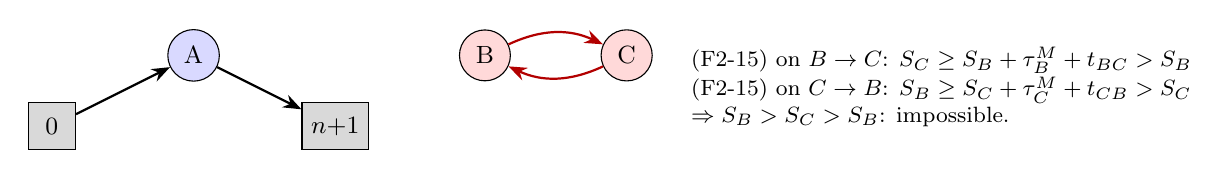
\begin{tikzpicture}[>=Stealth, every node/.style={font=\small}]
  \node[draw,fill=black!15,minimum size=6mm] (D0) at (0,0) {0};
  \node[circle,draw,fill=blue!15] (A) at (1.8,0.9) {A};
  \node[draw,fill=black!15,minimum size=6mm] (D1) at (3.6,0) {$n{+}1$};
  \node[circle,draw,fill=red!15] (B) at (5.5,0.9) {B};
  \node[circle,draw,fill=red!15] (C) at (7.3,0.9) {C};
  \draw[->,thick] (D0) -- (A); \draw[->,thick] (A) -- (D1);
  \draw[->,thick,red!70!black] (B) to[bend left=25] (C);
  \draw[->,thick,red!70!black] (C) to[bend left=25] (B);
  \node[align=left,font=\footnotesize] at (11.3,0.5) {(F2-15) on $B\to C$: $S_C\ge S_B+\tau^M_B+t_{BC}>S_B$\\(F2-15) on $C\to B$: $S_B\ge S_C+\tau^M_C+t_{CB}>S_C$\\$\Rightarrow S_B>S_C>S_B$: impossible.};
\end{tikzpicture}
\end{center}
Along any arc the start time strictly increases (charging and driving take positive time). Going round a loop would need $S_B>S_B$, so no loop can exist. This is the Miller--Tucker--Zemlin (MTZ) idea, with time playing the role of the ``position on the route''.

\without{A van could charge two EVs at once, teleport between EVs, or ``serve'' EVs on a loop it never reaches.}

\subsection{Time windows: start after the request, finish by $T$, measure lateness}
\begin{align}
S_i &\ge r_i && \forall i \tag{F2-17}\\
C_i &\le T && \forall i \tag{F2-18}\\
L_i &\ge C_i - l_i && \forall i \tag{F2-19}
\end{align}
\plain{(F2-17): no charging before the request; a van that arrives early waits. It is already implied by (F2-3) and is kept for readability. (F2-18): every car is fully charged within the horizon. This is a \emph{hard} rule and the second half of ``all requests satisfied''. (F2-19): lateness, see Section~\ref{sec:obj}. The desired time $l_i$ is \emph{soft}: missing it costs money but is allowed.}
\without{(F2-18) gone: the solver could push a hard EV beyond the evening and still call it ``served''.}

\subsection{Identical vans and variable types}
\begin{equation}
u_m \ge u_{m+1}\quad (m=1,\dots,|\M|-1);\qquad y,z,x,u,o\in\{0,1\},\quad S_i,L_i\ge0 \tag{F2-20, 21}
\end{equation}
\plain{Vans are interchangeable, so use them in index order: van 2 only if van 1 is used. Like (F2-7) this only removes duplicate solutions.}

\subsection{How the pieces work together for one EV}
\begin{center}
\renewcommand{\arraystretch}{1.25}
\begin{tabularx}{\textwidth}{@{}>{\raggedright\arraybackslash}p{3.2cm}XX@{}}
\toprule
 & \textbf{EV $i$ goes to an FCS gun $g$} & \textbf{EV $i$ is served by van $m$} \\
\midrule
assignment (F2-2) & $y_{ig}=1$, all $z_{im}=0$ & $z_{im}=1$, all $y_{ig}=0$ \\
earliest start & $S_i\ge r_i+t_{if}$ (F2-3) & $S_i\ge r_i$, $S_i\ge$ van arrival (F2-14/15) \\
waits for & the EV before it on the same gun (F2-4/5) & the van to finish the previous EV and drive over (F2-15) \\
duration & $\tau^F_i=E_i/22$ & $\tau^M_i=E_i/P^M$ \\
costs in $Z$ & $c^{EV}d_{if}$, $\pi^FE_i$ & its share of van km, $\pi^ME_i/\eta$ \\
both & \multicolumn{2}{l}{$c^Ww_i(C_i-r_i)$ and $c^Lw_iL_i$; must finish by $T$ (F2-18)} \\
\bottomrule
\end{tabularx}
\end{center}

%=====================================================================
\section{Worked example: 5 EVs, 1 station, 1 van}\label{sec:toy}

\subsection{Data}
One station $f$ at $(6,0)$ with 2 guns $g_1,g_2$; the depot at $(0,0)$; one van. Coordinates are in km, distances are straight lines, $T=4$\,h, all other values as in Section~\ref{sec:inputs}.

\begin{table}[h]
\centering
\renewcommand{\arraystretch}{1.15}
\begin{tabular}{@{}crrrrrrrrrr@{}}
\toprule
EV & location & $E_i$ & $r_i$ & $l_i$ & $R_i$ & $w_i$ & $\tau^F_i$ & $\tau^M_i$ & $d_{if}$ & reaches FCS? \\
\midrule
1 & $(-2,5)$ & 22 & 0 & 1.5 & 30 & 1.50 & 1.000 & 0.733 & 9.43 & yes \\
2 & $(8,2)$ & 11 & 0 & 1.0 & 20 & 2.00 & 0.500 & 0.367 & 2.83 & yes \\
3 & $(7,-3)$ & 22 & 0.5 & 2.0 & 25 & 1.75 & 1.000 & 0.733 & 3.16 & yes \\
4 & $(-5,4)$ & 15 & 0 & 1.5 & 4 & 2.80 & 0.682 & 0.500 & 11.71 & \textbf{no} ($11.71>4$) \\
5 & $(5,-1)$ & 22 & 0 & 1.5 & 30 & 1.50 & 1.000 & 0.733 & 1.41 & yes \\
\bottomrule
\end{tabular}
\caption{Toy instance. Times in hours, energy in kWh, distances in km.}\label{tab:toydata}
\end{table}

EV 4 has 4\,km of range and the station is 11.7\,km away, so $\G_4=\emptyset$ and (F2-2) forces it onto the van. The van will therefore go out anyway. The real question is: \emph{should the van also take one of the other EVs?}

\subsection{The optimal solution}
The instance was solved exactly by listing every feasible plan: every assignment of EVs to $g_1$, $g_2$ or the van, and every order on each resource, each started as early as allowed. There are 604 feasible plans. (For a fixed assignment and order, starting every session as early as possible is optimal, because all time terms in $Z$ grow with $C_i$.) The best plan has $Z^*=\Rs4589.16$:

\begin{center}
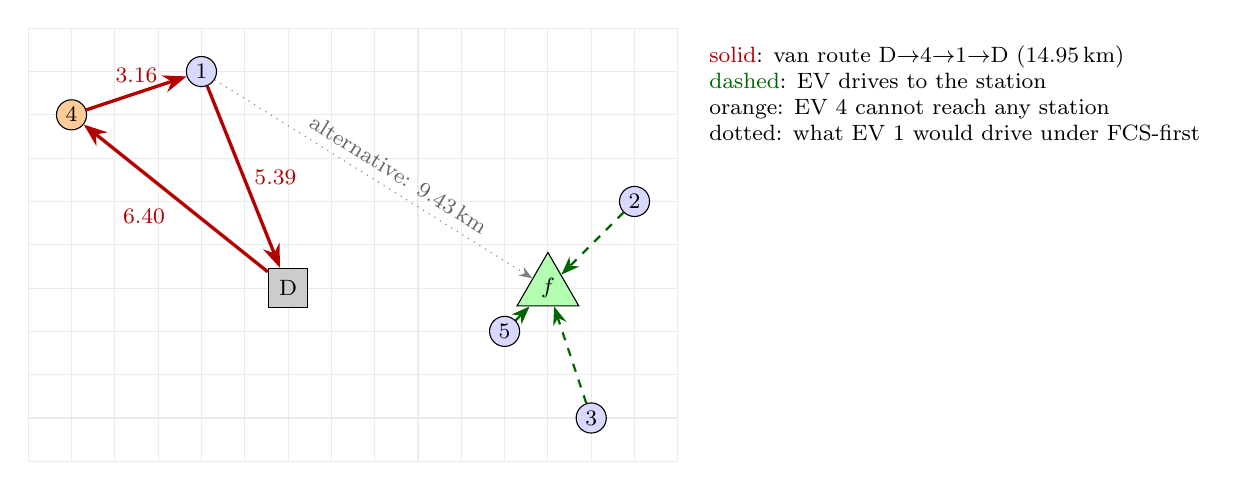
\begin{tikzpicture}[scale=0.55,>=Stealth, every node/.style={font=\footnotesize}]
  \draw[step=1,black!8] (-6,-4) grid (9,6);
  \node[draw,fill=black!20,minimum size=5mm] (D) at (0,0) {D};
  \node[regular polygon,regular polygon sides=3,draw,fill=green!30,inner sep=1pt] (f) at (6,0) {$f$};
  \node[circle,draw,fill=blue!15,inner sep=1.5pt] (e1) at (-2,5) {1};
  \node[circle,draw,fill=blue!15,inner sep=1.5pt] (e2) at (8,2) {2};
  \node[circle,draw,fill=blue!15,inner sep=1.5pt] (e3) at (7,-3) {3};
  \node[circle,draw,fill=orange!40,inner sep=1.5pt] (e4) at (-5,4) {4};
  \node[circle,draw,fill=blue!15,inner sep=1.5pt] (e5) at (5,-1) {5};
  \draw[->,very thick,red!70!black] (D) -- node[below left]{6.40} (e4);
  \draw[->,very thick,red!70!black] (e4) -- node[above]{3.16} (e1);
  \draw[->,very thick,red!70!black] (e1) -- node[right]{5.39} (D);
  \draw[->,thick,dashed,green!40!black] (e2) -- (f);
  \draw[->,thick,dashed,green!40!black] (e3) -- (f);
  \draw[->,thick,dashed,green!40!black] (e5) -- (f);
  \draw[->,dotted,black!50] (e1) -- node[pos=0.55,above,sloped,black!60]{alternative: 9.43\,km} (f);
  \node[anchor=west,align=left] at (9.5,4.5) {\textcolor{red!70!black}{solid}: van route D$\to$4$\to$1$\to$D (14.95\,km)\\\textcolor{green!40!black}{dashed}: EV drives to the station\\orange: EV 4 cannot reach any station\\dotted: what EV 1 would drive under FCS-first};
\end{tikzpicture}
\end{center}

\textbf{Variable values.} $y_{2,g_1}=y_{3,g_1}=1$, $y_{5,g_2}=1$; $z_{4m}=z_{1m}=1$; $x_{0,4,m}=x_{4,1,m}=x_{1,n+1,m}=1$; $u_m=1$; $o_{23}=1$ (EV 2 before EV 3 on $g_1$; the other $o_{ij}$ do not matter because those pairs do not share a gun); $L_1=0.116$, all other $L_i=0$.

\textbf{How the start times come out of the constraints.}
\begin{itemize}[leftmargin=1.4em,itemsep=1pt]
  \item EV 5 on $g_2$: (F2-3) $S_5\ge0+1.41/25=0.057$. Nothing else on $g_2$, so $S_5=0.057$, $C_5=1.057$.
  \item EV 2 on $g_1$: (F2-3) $S_2\ge 0.113$, so $S_2=0.113$, $C_2=0.613$.
  \item EV 3 on $g_1$ after EV 2: (F2-3) $S_3\ge0.5+0.126=0.626$; (F2-4) with $o_{23}=1$: $S_3\ge S_2+\tau^F_2=0.613$. So $S_3=0.626$, $C_3=1.626$.
  \item EV 4 first on the van: (F2-14) $S_4\ge t_{04}=6.40/25=0.256$, so $S_4=0.256$, $C_4=0.756$.
  \item EV 1 after EV 4: (F2-15) $S_1\ge S_4+\tau^M_4+t_{41}=0.256+0.5+0.126=0.883$, so $C_1=1.616$. That is $0.116$\,h after $l_1=1.5$, so $L_1=0.116$.
  \item Return: (F2-16) $1.616+5.39/25=1.831\le T=4$. Battery (F2-13): $(15+22)/0.9+0.25\times14.95=44.9\le150$ kWh. Capacity (F2-12): $2\le6$.
\end{itemize}

\subsection{Timeline (Gantt chart)}
\newcommand{\gbar}[5]{\fill[#4] (#1*6.5,#3-0.28) rectangle (#2*6.5,#3+0.28); \draw (#1*6.5,#3-0.28) rectangle (#2*6.5,#3+0.28); \node[font=\scriptsize] at ({(#1+#2)/2*6.5},#3) {#5};}
\newcommand{\gaxis}{%
  \foreach \t in {0,0.5,1,1.5,2} {\draw (\t*6.5,-0.55) -- (\t*6.5,-0.45); \node[below,font=\scriptsize] at (\t*6.5,-0.55) {\t\,h};}
  \draw[->] (0,-0.5) -- (2.15*6.5,-0.5);
  \node[left,font=\small] at (0,2) {gun $g_1$}; \node[left,font=\small] at (0,1) {gun $g_2$}; \node[left,font=\small] at (0,0) {van};}
\begin{center}
\textbf{Optimal plan} ($Z=\Rs4589$)\\[2pt]
\begin{tikzpicture}
  \gaxis
  \gbar{0.113}{0.613}{2}{blue!20}{EV 2}
  \gbar{0.626}{1.626}{2}{blue!20}{EV 3}
  \gbar{0.057}{1.057}{1}{blue!20}{EV 5}
  \gbar{0}{0.256}{0}{black!12}{}
  \gbar{0.256}{0.756}{0}{orange!40}{EV 4}
  \gbar{0.756}{0.883}{0}{black!12}{}
  \gbar{0.883}{1.616}{0}{blue!20}{EV 1}
  \gbar{1.616}{1.831}{0}{black!12}{}
  \draw[red,thick] (1.5*6.5,-0.35) -- (1.5*6.5,0.35); \node[red,font=\scriptsize,above] at (1.5*6.5,0.3) {$l_1$};
\end{tikzpicture}
\\[8pt]
\textbf{FCS-first plan} (every EV that can reach a station is sent there; $Z=\Rs4703$)\\[2pt]
\begin{tikzpicture}
  \gaxis
  \gbar{0.113}{0.613}{2}{blue!20}{EV 2}
  \gbar{0.613}{1.613}{2}{blue!20}{EV 1}
  \gbar{0.057}{1.057}{1}{blue!20}{EV 5}
  \gbar{1.057}{2.057}{1}{red!25}{EV 3 (queued)}
  \draw[red!70!black,thick,|-|] (0.626*6.5,1.38) -- (1.057*6.5,1.38) node[midway,above,font=\scriptsize]{EV 3 waits 0.43\,h};
  \gbar{0}{0.256}{0}{black!12}{}
  \gbar{0.256}{0.756}{0}{orange!40}{EV 4}
  \gbar{0.756}{1.012}{0}{black!12}{}
  \draw[red,thick] (2.0*6.5,0.65) -- (2.0*6.5,1.35); \node[red,font=\scriptsize,right] at (2.0*6.5,1.25) {$l_3$};
\end{tikzpicture}
\\[2pt]{\footnotesize grey = van driving, coloured = charging, orange = EV 4 (forced onto the van)}
\end{center}

\subsection{Why the van takes EV 1: the cost breakdown}
\begin{center}
\renewcommand{\arraystretch}{1.2}
\begin{tabular}{@{}lrrr@{}}
\toprule
\textbf{Term} & \textbf{FCS-first} & \textbf{F2 optimum} & \textbf{difference} \\
\midrule
$Z_1$ EV driving & 67.36 & 29.62 & $-37.74$ \\
$Z_2$ van driving & 192.09 & 224.26 & $+32.17$ \\
$Z_3$ dispatch & 1500.00 & 1500.00 & 0 \\
$Z_4$ energy & 848.23 & 918.39 & $+70.16$ \\
\midrule
\textbf{operating cost} $Z_1$--$Z_4$ & \textbf{2607.68} & \textbf{2672.27} & $\mathbf{+64.59}$ \\
\midrule
$Z_5$ inconvenience & 2014.40 & 1864.71 & $-149.69$ \\
$Z_6$ lateness & 80.61 & 52.18 & $-28.43$ \\
\midrule
\textbf{customer cost} $Z_5$--$Z_6$ & \textbf{2095.01} & \textbf{1916.89} & $\mathbf{-178.12}$ \\
\midrule
\textbf{total} $Z$ & \textbf{4702.69} & \textbf{4589.16} & $\mathbf{-113.53}$ \\
\bottomrule
\end{tabular}
\end{center}

\idea{The van does \emph{not} take EV 1 because EV 1 itself is much better off: EV 1 is ready at 1.616 by van against 1.613 at the station. It takes EV 1 because that \textbf{frees a gun for EV 3}. Under FCS-first, EV 1 occupies $g_1$ from 0.613, so EV 3 queues behind EV 5 on $g_2$ for 0.43\,h and finishes late. Putting EV 1 on the van costs \Rs64.59 more for the operator (extra van km and dearer van energy, minus EV 1's saved drive) but saves the drivers \Rs178.12 in waiting and lateness.}

This is exactly the effect a model without a clock cannot see. A capacity-only model like F4 only checks that the total charging hours fit at the station: $1+0.5+1+1=3.5\le2\times4=8$ hours. By that check the station has plenty of room, so nothing tells it to move EV 1. Only a model that schedules each gun in time (Idea 3) sees EV 3 waiting.

\subsection{How big is this model?}
\begin{tabular}{@{}ll@{}}
$y_{ig}$ & 4 reachable EVs $\times$ 2 guns $=8$ \\
$z_{im}$ & $5\times1=5$ \\
$x_{ijm}$ & $6\times6$ arcs (from $0$ or an EV, to an EV or $n{+}1$) $-$ 5 self-loops $-$ arc $0\to n{+}1$ $=30$ \\
$u_m$ & 1 \\
$o_{ij}$ & pairs of EVs that can share a gun: $\binom{4}{2}=6$ \\
\textbf{total} & \textbf{50 binaries}, plus 10 continuous ($S_i$, $L_i$) \\
\end{tabular}

Binaries grow fast: roughly $n^2|\M|$ for the van arcs and up to $n^2/2$ for the gun-order pairs. That is why F2 notes that $n\le25$--$50$ is realistic for Gurobi/CPLEX, and why larger instances need the size reductions in F2 Section 9 (nearest stations only, drop pairs that can never meet, or the capacity cut (F2-6) alone).

%=====================================================================
\section{One-page summary}\label{sec:cheat}

F2 Section 8 (``The complete model'') prints the whole MILP in one block. The table below gives the same model with one line of meaning per constraint.

\begin{center}
\renewcommand{\arraystretch}{1.3}
\small
\begin{tabularx}{\textwidth}{@{}l>{\raggedright\arraybackslash}p{6.6cm}X@{}}
\toprule
\textbf{Eq.} & \textbf{Formula (short)} & \textbf{Meaning} \\
\midrule
F2-1 & $\min Z_1+\dots+Z_6$ & EV km, van km, dispatch, energy, priority-weighted waiting, lateness \\
F2-2 & $\sum_g y_{ig}+\sum_m z_{im}=1$ & one resource per EV; no reachable station $\Rightarrow$ van \\
F2-3 & $S_i\ge r_i+\sum_f t_{if}Y_{if}$ & FCS start after request + drive \\
F2-4/5 & disjunctive pair with $o_{ij}$, big-M $T+\tau^F$ & same gun $\Rightarrow$ one after the other \\
F2-6 & $\sum_i\tau^F_iy_{ig}\le T-\min(r_i+t_{if})$ & optional cut: work fits on the gun \\
F2-7 & $\sum_iy_{ig_1}\ge\sum_iy_{ig_2}$ & optional: identical guns \\
F2-8/9 & out of 0 $=u_m$, into $n{+}1$ $=u_m$ & van leaves and returns once \\
F2-10/11 & in-arcs $=$ out-arcs $=z_{jm}$ & each van EV visited once by its van \\
F2-12 & $\sum_iz_{im}\le Q_mu_m$ & max EVs per van \\
F2-13 & $\sum_iE_iz_{im}/\eta+\beta\sum d_{ij}x_{ijm}\le B_mu_m$ & battery: delivered (with losses) + driving \\
F2-14 & $S_j\ge t_{0j}x_{0jm}$ & first EV after the drive from the depot \\
F2-15 & $S_j\ge S_i+\tau^M_i+t_{ij}-M(1-x_{ijm})$ & one EV at a time; removes subtours (MTZ) \\
F2-16 & $S_i+\tau^M_i+t_{i,n+1}\le T+\dots(1-x_{i,n+1,m})$ & back at the depot by $T$ \\
F2-17 & $S_i\ge r_i$ & not before the request \\
F2-18 & $C_i\le T$ & everyone fully charged by $T$ (hard) \\
F2-19 & $L_i\ge C_i-l_i$, $L_i\ge0$ & lateness beyond desired time (soft) \\
F2-20/21 & $u_m\ge u_{m+1}$; domains & identical vans; variable types \\
\bottomrule
\end{tabularx}
\end{center}

\subsection*{F2 against the project brief}
\begin{center}
\renewcommand{\arraystretch}{1.2}
\small
\begin{tabularx}{\textwidth}{@{}>{\raggedright\arraybackslash}p{6.4cm}X@{}}
\toprule
\textbf{Brief says} & \textbf{F2 does it with} \\
\midrule
Each EV assigned to exactly one resource & F2-2 \\
FCS cannot exceed capacity (2 guns) & one machine per gun, F2-4/5 (exact, in continuous time) \\
MCS has limited battery & F2-13 (delivered energy with losses + driving) \\
MCS max service capacity / 1 EV at a time & F2-12 / F2-15 \\
MCS start and end at the depot & nodes $0$, $n{+}1$, F2-8/9, F2-16 \\
Each MCS EV visited exactly once & F2-10/11 \\
Cost: EV travel, MCS travel, MCS operating cost & $Z_1$, $Z_2$, $Z_3$ (+ energy $Z_4$) \\
Customer inconvenience as a penalty & $Z_5$ (priority-weighted waiting) + $Z_6$ (lateness) \\
All requests satisfied & F2-2 + F2-18 \\
(Mixed) integer linear program & every term and constraint is linear \\
\bottomrule
\end{tabularx}
\end{center}

\subsection*{Things to keep in mind when you implement F2}
\begin{itemize}[leftmargin=1.4em,itemsep=2pt]
  \item \textbf{Infeasible = fleet too small.} Because F2-18 is hard, an instance with too few vans or guns has no solution at all. For experiments, add an ``unserved'' binary $s_i$ to F2-2 ($\dots+s_i=1$) with a large penalty, and report how many EVs are unserved. This is also what F3 does.
  \item \textbf{Report $Z$ with and without the constant} $c^W\sum_iw_ir_i$, and always report $Z_1$--$Z_4$ and $Z_5$--$Z_6$ separately, as in the table above. The brief's main KPI is operating cost.
  \item \textbf{Start small.} Check your code on this toy instance first: it must give $Z^*=4589.16$ with the plan shown here.
  \item \textbf{Assumptions F2 makes} (state them in the report): all requests known at time 0; constant charging power; no partial charging; vans are not recharged during the horizon; one speed for all travel; vans leave the depot at time 0 (leaving later is the same as waiting at the first EV).
  \item \textbf{What F2 does not include:} time-of-use prices (that is F3, S2 and S4), dynamic requests, congestion.
\end{itemize}

\end{document}
